\documentclass[12pt,a4paper]{article}
\usepackage{fullpage}
\usepackage[utf8]{inputenc}
\usepackage{amsmath}
\usepackage{amsfonts}
\usepackage{amssymb}
\usepackage{enumerate}
\usepackage{enumitem}
\usepackage{graphicx}

\setlist{nosep}

\begin{document}

%\title{CSCI 4448: Object Oriented Analysis and Design\\ Project Part 2}
%\date{October 19, 2015}        
%\maketitle

\noindent\textbf{Project Part 2}

\paragraph{Team:}Andrew Gordon, Tommy Hoffmann, Connor McGuinness, Daniel Zurawski

\paragraph{Title:}What To Wear Weather

\paragraph{Project Summary:}Android application which tells users what kind
of clothes they should be wearing based on the weather in their local area.
\\

\noindent\textbf{Requirements:}
\\\\
%insert tables here
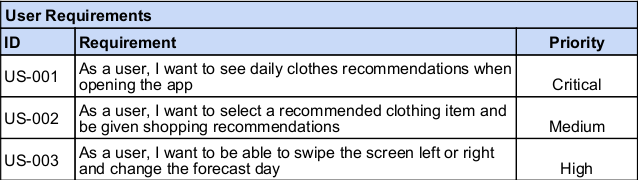
\includegraphics[scale=0.7]{user.png}\\\\
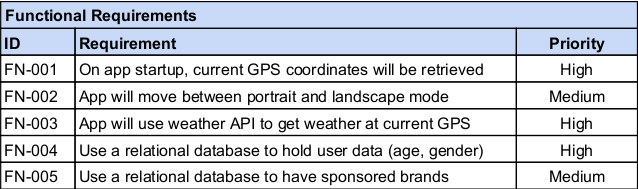
\includegraphics[scale=0.7]{functional.png}\\\\
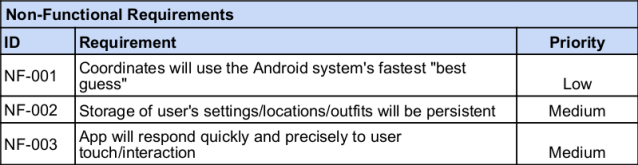
\includegraphics[scale=0.7]{non-functional.png}\\\\

\noindent\textbf{Users and Tasks:} \\\\
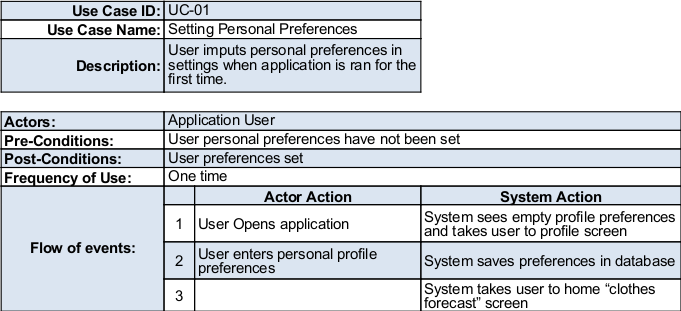
\includegraphics[scale=0.7]{usecase1.png} \\\\
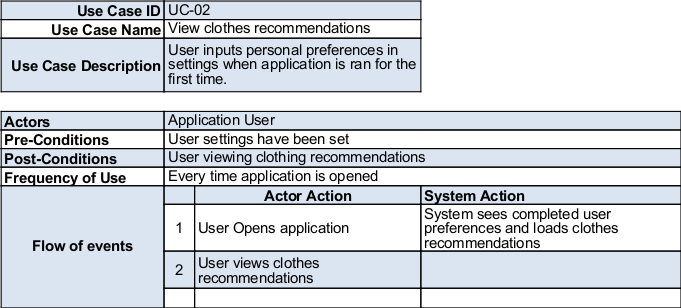
\includegraphics[scale=0.7]{usecase2.png} \\\\
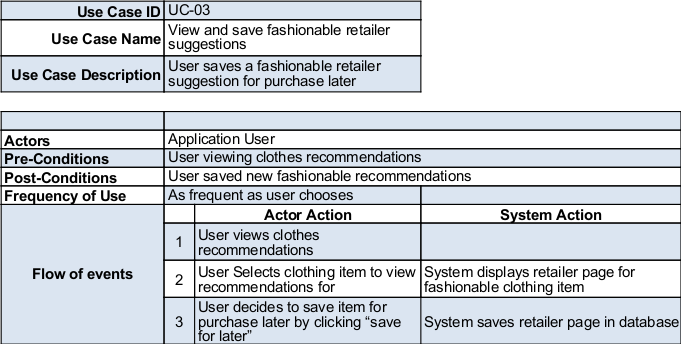
\includegraphics[scale=0.7]{usecase3.png} \\\\
%insert use case diagrams

\paragraph{Activity Diagram:}
%activity of most complex use case

\paragraph{Data Storage:} The application will use the Android internal storage in XML format.
The storage requirements are not very large, in paticular user preferences and saved clothing recommendations
will needed to be storaged, which we anticipate will be a few dozen items. The User Preferences class and User Recommendation class will be retrieving and modifying data from data storage.

\paragraph{UI Mockups:}

\paragraph{User Interactions:}

\paragraph{Class Diagram}
\end{document}
